\chapter{Trabalhos Relacionados}
\label{cap:trabalhos-relacionados}

  A visualização de dados de tráfego tem um amplo histórico e se divide em
algumas sub áreas. As pesquisas que julgamos relevantes tocam as áreas de
visualização da informação - \emph{InfoViz}, cujo foco é desvendar novos métodos
para visualizar uma informação, como \emph{bundling}, e também a área de análise
visual aplicada - \emph{Visual Analytics}, que se aproxima mais a sistemas e
soluções utilizadas em ambientes do mundo real. Ambos trabalhos trazem
contribuições em diferentes níveis para a nossa pesquisa.

O primeiro trabalho que destacamos é o de \citet{Zhou2013}.
Sua pesquisa é uma revisão teórica sobre diferentes modelos de \emph{bundling},
dentre eles, os primeiros métodos baseados em algoritmos de processamento de
imagem (linhagem que gerou o \emph{KDEEB} utilizado no \emph{CUBu}). Esse trabalho reforça o
\emph{bundling} como uma técnica promissora para a visualização de grandes
quantidades de dados com aplicações na visualização de mapas de fluxos (com
dados de mobilidade), visualização de grafos e redes de conexão, gráficos de
coordenadas paralelas e basicamente qualquer tipo de visualização baseadas em
linhas.

\citet{Lhuillier2017} traz uma revisão mais recente sobre
o \emph{bundling}. Os autores sugerem ainda uma definição formal sobre a operação de
\emph{bundling} em um conjunto de dados, e a partir daí listam as
características, objetivos e limitações de uso ao lidar com dados espaciais
(como dados de mobilidade) e também outros tipos de dados sem relação espacial
(grafos, coordenadas paralelas). O resultado é uma visão geral sobre o estado da
arte em cada um desses segmentos. Dentre suas contribuições está uma nova
taxonomia (Figura~\ref{table:bundling-methods}) para a ajudar pesquisadores e
usuários a selecionarem os algoritmos de \emph{bundling} com base no tipo de
dado. 

 \begin{figure}[!htb]
  \centering
  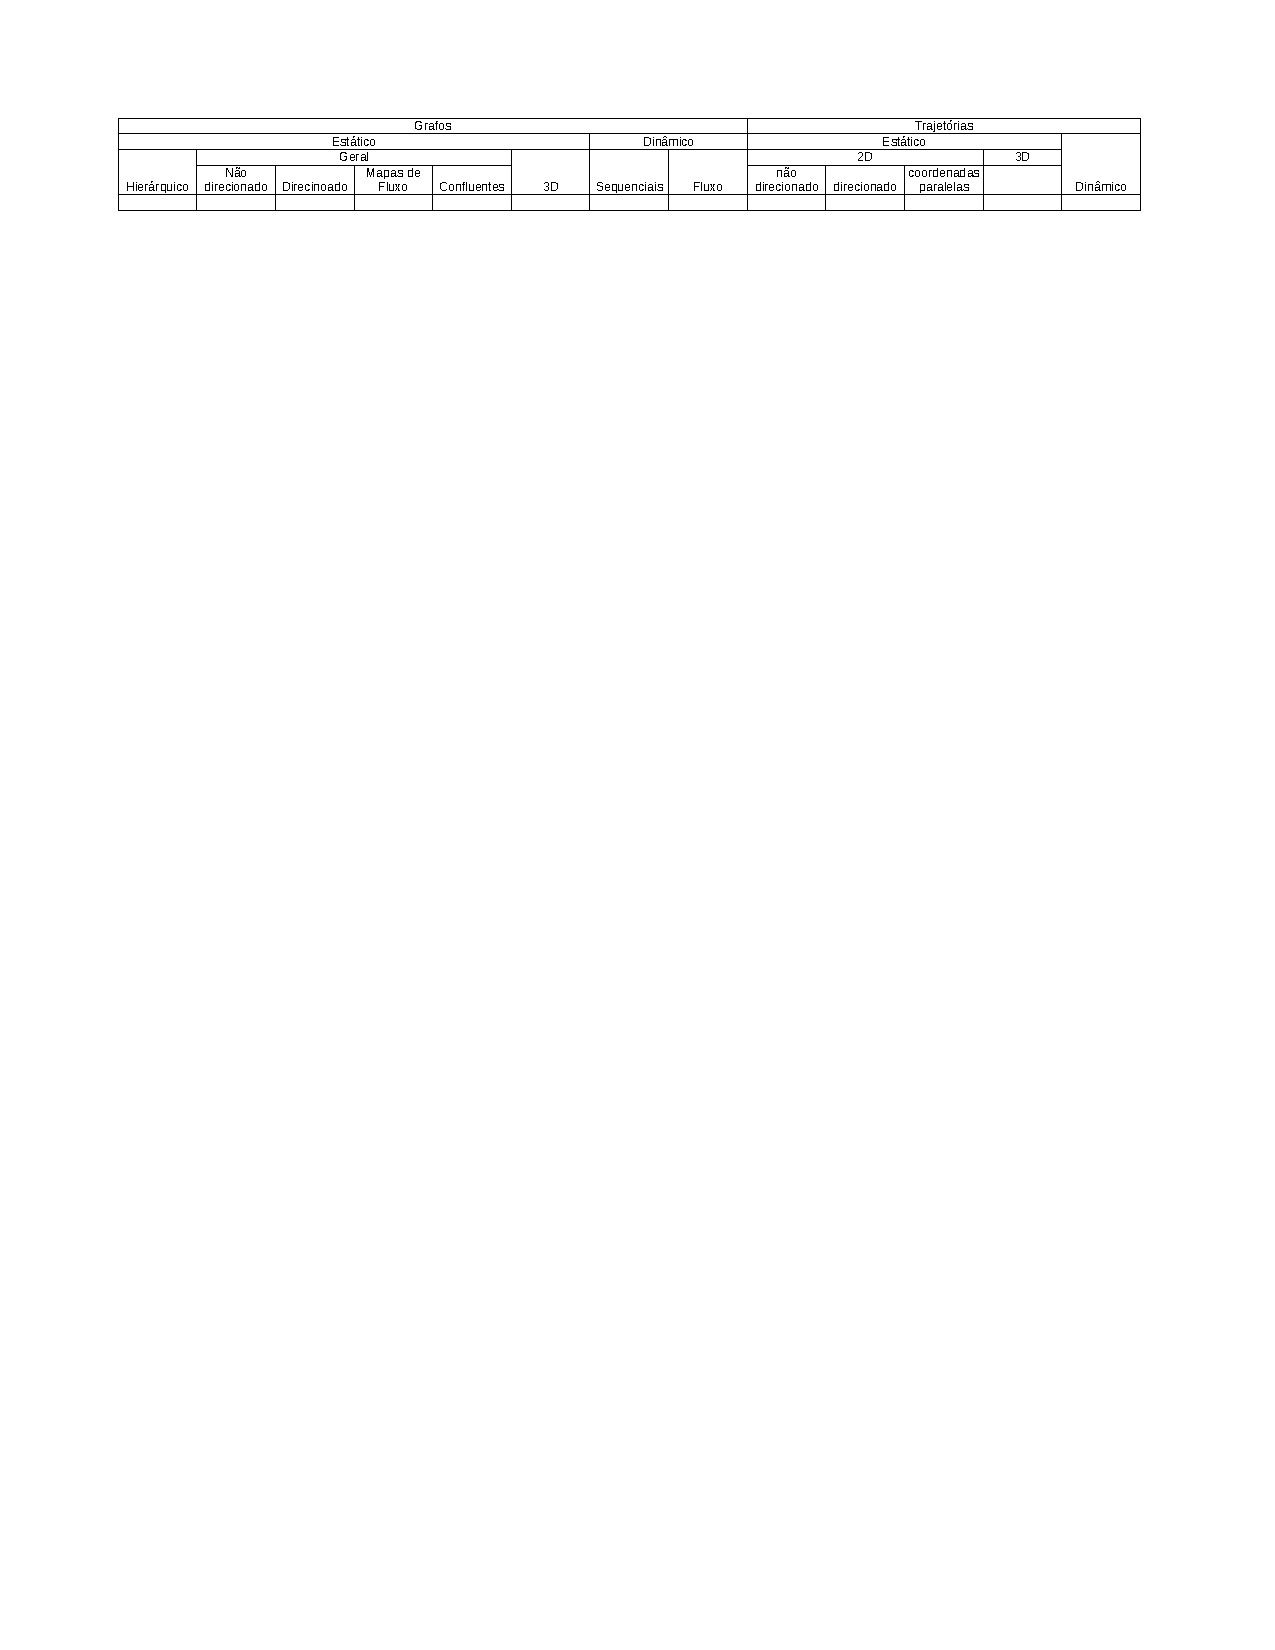
\includegraphics[width=\textwidth]{../figuras/estado-da-arte.pdf}
  \caption[Taxonomia dos métodos de \emph{bundling} baseado no tipo de dado]{Taxonomia dos métodos de \emph{bundling} baseado no tipo de dado. Fonte: \citet{Lhuillier2017}}
   \label{table:bundling-methods}
 \end{figure}

Igualmente relevante, \citet{Telea2018} apresenta uma rica revisão geral das
áreas de visualização científica e de processamento de imagem, apontando métodos
utilizados nessas áreas que beneficiaram a visualização de grandes grafos
multivariados e complexos. Ele mostra com detalhes a história evolutiva das
técnicas de \emph{bundling} até o estado da arte atual, representado por métodos como o
\emph{CUBu}, que permitiram a visualização interativa de grandes grafos com
milhares de elementos. Além disso eles também citam alguns dos desafios em
aberto, como por exemplo, a dificuldade de avaliar a qualidade do
\emph{bundling}, já que não há uma maneira objetiva que diga o quão correto está
um determinado resultado.

Duas outras importantes fontes são \citet{Chen2015} e
\citet{Andrienko2017Visual}, que também fazem uma revisão da literatura e
apresentam diversos trabalhos sobre análises de dados do tráfego e de mobilidade
em geral. Nesse levantamento eles discutem questões sobre coleta e tipos de
dados, uso de técnicas de visualização apropriadas para diferentes objetivos de
análise, entre outros conceitos. Os dois trabalhos abrangem em suas revisões
pesquisas de vários contextos, como análise de incidentes no tráfego,
monitoramento de veículos em tempo real, detecção de congestionamentos, sugestão
de rotas e outras atividades executadas por usuários e especialistas de
transporte. A partir desses dois estudos obtemos muitos insumos para
complementar o conhecimento sobre a área de visualização e análise de dados de
transporte em geral e enriquecer nossa revisão da literatura. Pudemos
utilizá-los como referência para parte dos conceitos teóricos apresentados na
Seção \ref{sec:dados-de-trajetorias} e também como ponte para outras pesquisas
na área. Âmbos, \citet{Chen2015} e \citet{Andrienko2017Visual}, relacionam o
\emph{bundling} na categoria de soluções para visualização de fluxos de
mobilidade, pontuando-o como uma boa alternativa para visualização de grandes
quantidades de dados, além também de levantar seu principal efeito colateral de
distorção espacial dos dados, apontando que isso pode influenciar ou dificultar
a análise dos resultados, porém não se aprofundam muito no assunto.

Outros trabalhos também levantam a questão da distorção espacial dos dados 
causadas pelo \emph{bundling} e propõem abordagens alternativas 
que não modificam os caminhos originais das trajetórias;
\citet{Landersberg2016} mostra uma representação em linhas do tráfego sobre um
mapa e apresenta algoritmos de clusterização para agrupar o tráfego por regiões
e também no tempo, reduzindo a oclusão do desenho. Sua análise é focada em
destacar diferentes momentos onde há mudanças significativas nos fluxos. O
desafio de sua técnica é estabelecer métricas que capturam esses momentos.  Eles
apresentam um sistema interativo e verificam seu método com dados de
\emph{tweets} geolocalizados na cidade de Londres e também de redes de
celulares. Fulano apresenta uma visualização de matrizes, argumentando também
que esse é um modelo visual que contorna a distorção e interpretação de
visualizações com \emph{bundling}. E Ciclano apresenta uma visualização em
linhas que estima a densidade de fluxo para cada par de locais por um modelo de
densidade baseado em vetor. Em seguida, um subconjunto de caminhos suavizados é
selecionado para representar o fluxo principal no mapa de fluxo. A Fig. 9 mostra
os fluxos de imigração gerados por esta abordagem.

De fato este efeito colateral do \emph{bundling} sobre a alteração espacial dos
dados merece a devida atenção, no entanto isto não chega a ser exatamente um
problema; \emph{Frameworks} como o \emph{CUBu} apresentam recursos para mitigar
confusões causadas por este efeito, como por exemplo, a capacidade de controlar
o efeito do bundling  através do parâmetro $k$ (tamanho do \emph{kernel}), e a
capacidade de desfazer o bundling parcial ou totalmente, restaurando as
trajetórias para a posição inicial, através da interpolação dos resultados com a
posição original \citep{zwan:16}. Embora isso requeira um pouco mais de
esforço cognitivo, tais recursos permitem que usuários possam compreender
completamente o modelo visual e interpretar o resultado. Outro ponto em favor do
\emph{bundling} é que ele foi testado de maneira relevante em grandes conjuntos
de dados com centenas de milhares de dados, como posto em \citet{Telea2018,
Lhuillier2017}, o que não necessariamente é atestado para outros métodos que
citamos, segundo a nossa revisão da literatura.

Dentre outras pesquisas que utilizam bundling para análise de movimentação,
\citet{Anita2017} criou uma visualização com \emph{bundling} para
estudar características da migração de aves. \citet{Klein2014} desenvolveu uma
visualização dinâmica para mostrar variações do tráfego aéreo ao longo do tempo
e \citep{Willems2009} fez uma análise da movimentação de embarcações marítimas
também explorando técnicas de \emph{bundling}. Separadamente,
\citep{Blascheck2017} mostra como a técnica foi empregada para simplificar a
visualização de dados de monitoramento da visão para inferir padrões de leitura.

\citet{zeng:19} adaptaram o método KDEEB para restringir o \emph{bundling}
ao longo da rede de vias da cidade as quais os dados das trajetórias forma
coletados no que eles denominaram \emph{Road Aware Edge
Bundling (RAEB)}. Sua técnica foi demonstrada em dados contendo
166 mil viagens de táxi da cidade de Nova Iorque. RAEB é o único o único
trabalho que utiliza \emph{bundling} com dados de mobilidade de que estamos cientes.
No entanto, ele requer dados detalhados das trajetórias (não apenas OD) e também
dados do leiaute das vias da cidade.


% \citet{Klein2014} faz uma análise do tráfego aéreo
% da França para detectar as conexões entre os diferentes aeroportos, pontos de
% congestionamentos e permitir uma exploração com base em vários atributos, como
% direção e altitude dos voos, além de uma janela de tempo que permite navegar
% entre diferentes instantes do tráfego. Eles utilizam o algoritmo de
% \emph{bundling} KDEEB para reduzir a oclusão na visualização das trajetórias
% e apresentam uma interpolação das trajetórias sem \emph{bundling} para visualizar
% sua direção, já que o KDEEB não inclui atributos como direção no processo de \emph{bundling}.


% \citet{Anita2017} apresenta uma técnica de \emph{bundling}, resultado de uma
% otimização do algoritmo FDEB, criado por \citet{Selassie2011}. Para isso,
% utilizam uma etapa de clusterização aplicada previamente nos dados, e
% posteriormente aplicam o \emph{bundling} em cada cluster. Eles testaram sua
% abordagem em vários conjuntos de dados com informações da migração de pessoas
% entre regiões dos EUA, migração de pássaros e viagens de aviões, mostrando um
% ganho entre 30\% até 50\% no desempenho do algoritmo. A vantagem da sua
% abordagem é que ela pode ser utilizada em conjunto com outros métodos de
% \emph{bundling}. 

---------------------

Não menos importante, alguns outros trabalhos que pesquisamos mostram resultados
interessantes a respeito da visualização e análise de dados de mobilidade e seus
atributos e também valem ser citados, como \citet{Ferreira2013}, que fazem uma
análise de origem e destino de 500 mil viagens de táxi feitas em um dia na
cidade de Nova Iorque. Sua visualização é baseada em pontos que destacam as
origens e destinos das viagens com cores diferentes. O resultado é similar a um
mapa de densidades que mostra a distribuição das viagens sobre a cidade. Eles
também implementam uma estratégia robusta de organização dos dados na memória
para permitir que os usuários façam buscas e apliquem filtros em uma grande
quantidade de dados de maneira interativa.

\citet{Chu2014} também faz uma análise das trajetórias de milhares de viagens
de táxi em uma grande cidade na China para descobrir relações entre as rotas
utilizadas e relações entre ruas. Eles fazem uma transformação das latitudes e
longitudes para o nome das ruas por onde os veículos se locomovem e aplicam métodos de
clusterização e análise de texto que dão uma visão semântica das relações entre
as vias que compõe a malha rodoviária da cidade. Os resultados são mostrados em
um painel com vários tipos de visualização que utiliza mapas, gráficos e outros
recursos para exploração dos dados. \citet{Guo2011} criaram um sistema chamado
TripVista que mostra o tráfego em três perspectivas através de um painel
iterativo.  Seu sistema é focado em mostrar detalhes em nível microscópico
sobre o tráfego em cruzamentos entre ruas da cidade, como direção, quantidade
de veículos e também anomalias de motoristas que trafegam na direção contrária
da permitida. 

Por último \citet{Kim2018} utilizam o que eles chamam de \emph{campos
gravitacionais} para construir um mapa de fluxo de dados geoespaciais
analisando apenas as informações estatísticas da distribuições dos pontos ao
longo do tempo. Sua abordagem, no entanto implica uma série de restrições
estatísticas nos dados, como número mínimo de amostras e distribuição uniforme
dos dados ao longo do tempo.

Em nossa revisão, buscamos obter um panorama geral das lacunas que podem ser
preenchidas em relação ao uso de \emph{bundling} na visualização de fluxos de
mobilidade urbana. Para sumarizar o conteúdo de nossa revisão, mostramos na
Tabela~\ref{table:trabalhos} a seguir uma lista dos trabalhos em ordem
cronológica indicando algumas características sobre o tipo de dado analisado,
presença do \emph{bundling} na construção da solução e leiaute da visualização.
Essas informações colaboram na visão do geral dos trabalhos que se relacionam
com a nossa pesquisa.

\begin{table}[htb!]
\begin{tabular}{|M{0.58}|M{0.11}|M{0.115}|M{0.09}|}
\hline
\textbf{Trabalho}       & \textbf{Dados do Trânsito} & \textbf{\emph{Bundling}} & \textbf{Leiaute}  \\ \hline
Nossa proposta          & \checkmark                 & \checkmark               &          linhas   \\ \hline
\citet{Kim2018}         & x                          &  x                       &          linhas   \\ \hline
\citet{Andrienko2017}   & \checkmark                 &  x                       &          radial   \\ \hline
\citet{Anita2017}       & x                          & \checkmark               &          linhas   \\ \hline
\citet{Landersberg2016} & x                          &  x                       &          linhas   \\ \hline
\citet{Klein2014}       & x                          & \checkmark               &          linhas   \\ \hline
\citet{Chu2014}         & x                          &  x                       &          variado  \\ \hline
\citet{Ferreira2013}    & \checkmark                 &  x                       &          pontos   \\ \hline
\citet{Zeng2013}        & x                          & \checkmark               &          radial   \\ \hline
\citet{Guo2011}         & \checkmark                 &  x                       &          variado  \\ \hline

\end{tabular}
\caption[Lista de trabalhos relacionados]{Lista de trabalhos relacionados. \label{table:trabalhos}}
\end{table}

Concluímos que as formas de visualizar os dados de mobilidade utilizando
técnicas de \emph{bundling} ainda possuem pontos a ser explorados. Nossa
abordagem contempla um novo cenário para utilização das técnicas de
\emph{bundling} na análise de fluxos de mobilidade urbana. Além de contribuímos
com uma análise singular do contexto de mobilidade urbana na cidade de São
Paulo, nós avançamos também na investigação da particularidades do \emph{CUBu}
ao adaptá-lo para este contexto, em que se diz respeito ao seu potencial de uso
e ajuste de parâmetros. No próximo capítulo apresentamos a metodologia para o
desenvolvimento de nossa proposta.